\documentclass[a4paper,5pt]{amsbook}
%%%%%%%%%%%%%%%%%%%%%%%%%%%%%%%%%%%%%%%%%%%%%%%%%%%%%%%%%%%%%%%%%%%%%

\usepackage{booktabs}
\usepackage{graphicx}
\usepackage{multicol}
% \usepackage[]{float}
\usepackage{amssymb}
% \usepackage{amsfonts}
% \usepackage[]{amsmath}
% \usepackage[]{epsfig}
% \usepackage[brazil]{babel}
% \usepackage[utf8]{inputenc}
% \usepackage{verbatim}
%\usepackage[]{pstricks}
%\usepackage[notcite,notref]{showkeys}
\usepackage{subcaption}
\usepackage[inline]{enumitem}

%%%%%%%%%%%%%%%%%%%%%%%%%%%%%%%%%%%%%%%%%%%%%%%%%%%%%%%%%%%%%%

\newcommand{\sen}{\,\mbox{sen}\,}
\newcommand{\tg}{\,\mbox{tg}\,}
\newcommand{\cosec}{\,\mbox{cosec}\,}
\newcommand{\cotg}{\,\mbox{cotg}\,}
\newcommand{\ds}{\displaystyle}

%%%%%%%%%%%%%%%%%%%%%%%%%%%%%%%%%%%%%%%%%%%%%%%%%%%%%%%%%%%%%%%%%%%%%%%%

\setlength{\textwidth}{16cm} \setlength{\topmargin}{-2cm}
\setlength{\textheight}{25cm}
\setlength{\leftmargin}{1.2cm} \setlength{\rightmargin}{1.2cm}
\setlength{\oddsidemargin}{0cm}\setlength{\evensidemargin}{0cm}

%%%%%%%%%%%%%%%%%%%%%%%%%%%%%%%%%%%%%%%%%%%%%%%%%%%%%%%%%%%%%%%%%%%%%%%%

% \renewcommand{\baselinestretch}{1.6}
% \renewcommand{\thefootnote}{\fnsymbol{footnote}}
% \renewcommand{\theequation}{\thesection.\arabic{equation}}
% \setlength{\voffset}{-50pt}
% \numberwithin{equation}{chapter}

%%%%%%%%%%%%%%%%%%%%%%%%%%%%%%%%%%%%%%%%%%%%%%%%%%%%%%%%%%%%%%%%%%%%%%%

\begin{document}
\thispagestyle{empty}
\hspace{-0.6cm}
\begin{minipage}[p]{0.14\linewidth}
	\includegraphics[scale=0.24]{ufgd.png}
\end{minipage}
\begin{minipage}[p]{0.7\linewidth}
\begin{tabular}{c}
\toprule{}
{{\bf UNIVERSIDADE FEDERAL DA GRANDE DOURADOS}}\\
{{\bf Prof.\ Adriano Barbosa}}\\

{{\bf C\'alculo 2 --- Avalia\c{c}\~ao P2}}\\

\midrule{}
Matem\'atica\hspace{5cm}29 de Mar\c{c}o de 2017 \\
\bottomrule{}
\end{tabular}
\vspace{-0.45cm}
%
\end{minipage}
\begin{minipage}[p]{0.15\linewidth}
\begin{flushright}
\def\arraystretch{1.2}
\begin{tabular}{|c|c|}  % chktex 44
\hline\hline  % chktex 44
1 & \hspace{1.2cm} \\
\hline  % chktex 44
2& \\
\hline  % chktex 44
3& \\
\hline  % chktex 44
4&  \\
\hline  % chktex 44
5&  \\
\hline  % chktex 44
{\small Total}&  \\
\hline\hline  % chktex 44
\end{tabular}
\end{flushright}
\end{minipage}

%------------------------
\vspace{0.5cm}
{\bf Aluno(a):}\dotfill{}  % chktex 36
%----------------------------

\vspace{0.2cm}
%%%%%%%%%%%%%%%%%%%%%%%%%%%%%%%%   formulario  inicio  %%%%%%%%%%%%%%%%%%%%%%%%%%%%%%%%
\begin{enumerate}
	\vspace{0.5cm}
	\item Calcule a integral $\ds\int \frac{\sqrt{x^2-4}}{x}\ dx$.

	\vspace{0.5cm}
	\item Dados os polin\^omios $p(x) = 10$ e $q(x) = 5x^2-2x^3$:
		\begin{enumerate}
			\vspace{0.3cm}
			\item Fatore o polin\^omio $q(x)$.
			\vspace{0.3cm}
			\item Escreva $\ds\frac{p(x)}{q(x)}$ como soma de fra\c{c}\~oes parciais.
			\vspace{0.1cm}
			\item Calcule a integral $\ds\int\frac{p(x)}{q(x)}\ dx$.
		\end{enumerate}

	\vspace{0.5cm}
	\item Determine se a integral impr\'opria $\ds\int_1^\infty \frac{\ln{x}}{x}\ dx$ \'e convergente ou divergente.

	\vspace{0.5cm}
	\item Calcule a \'area da figura abaixo:
		\begin{figure}[h]
			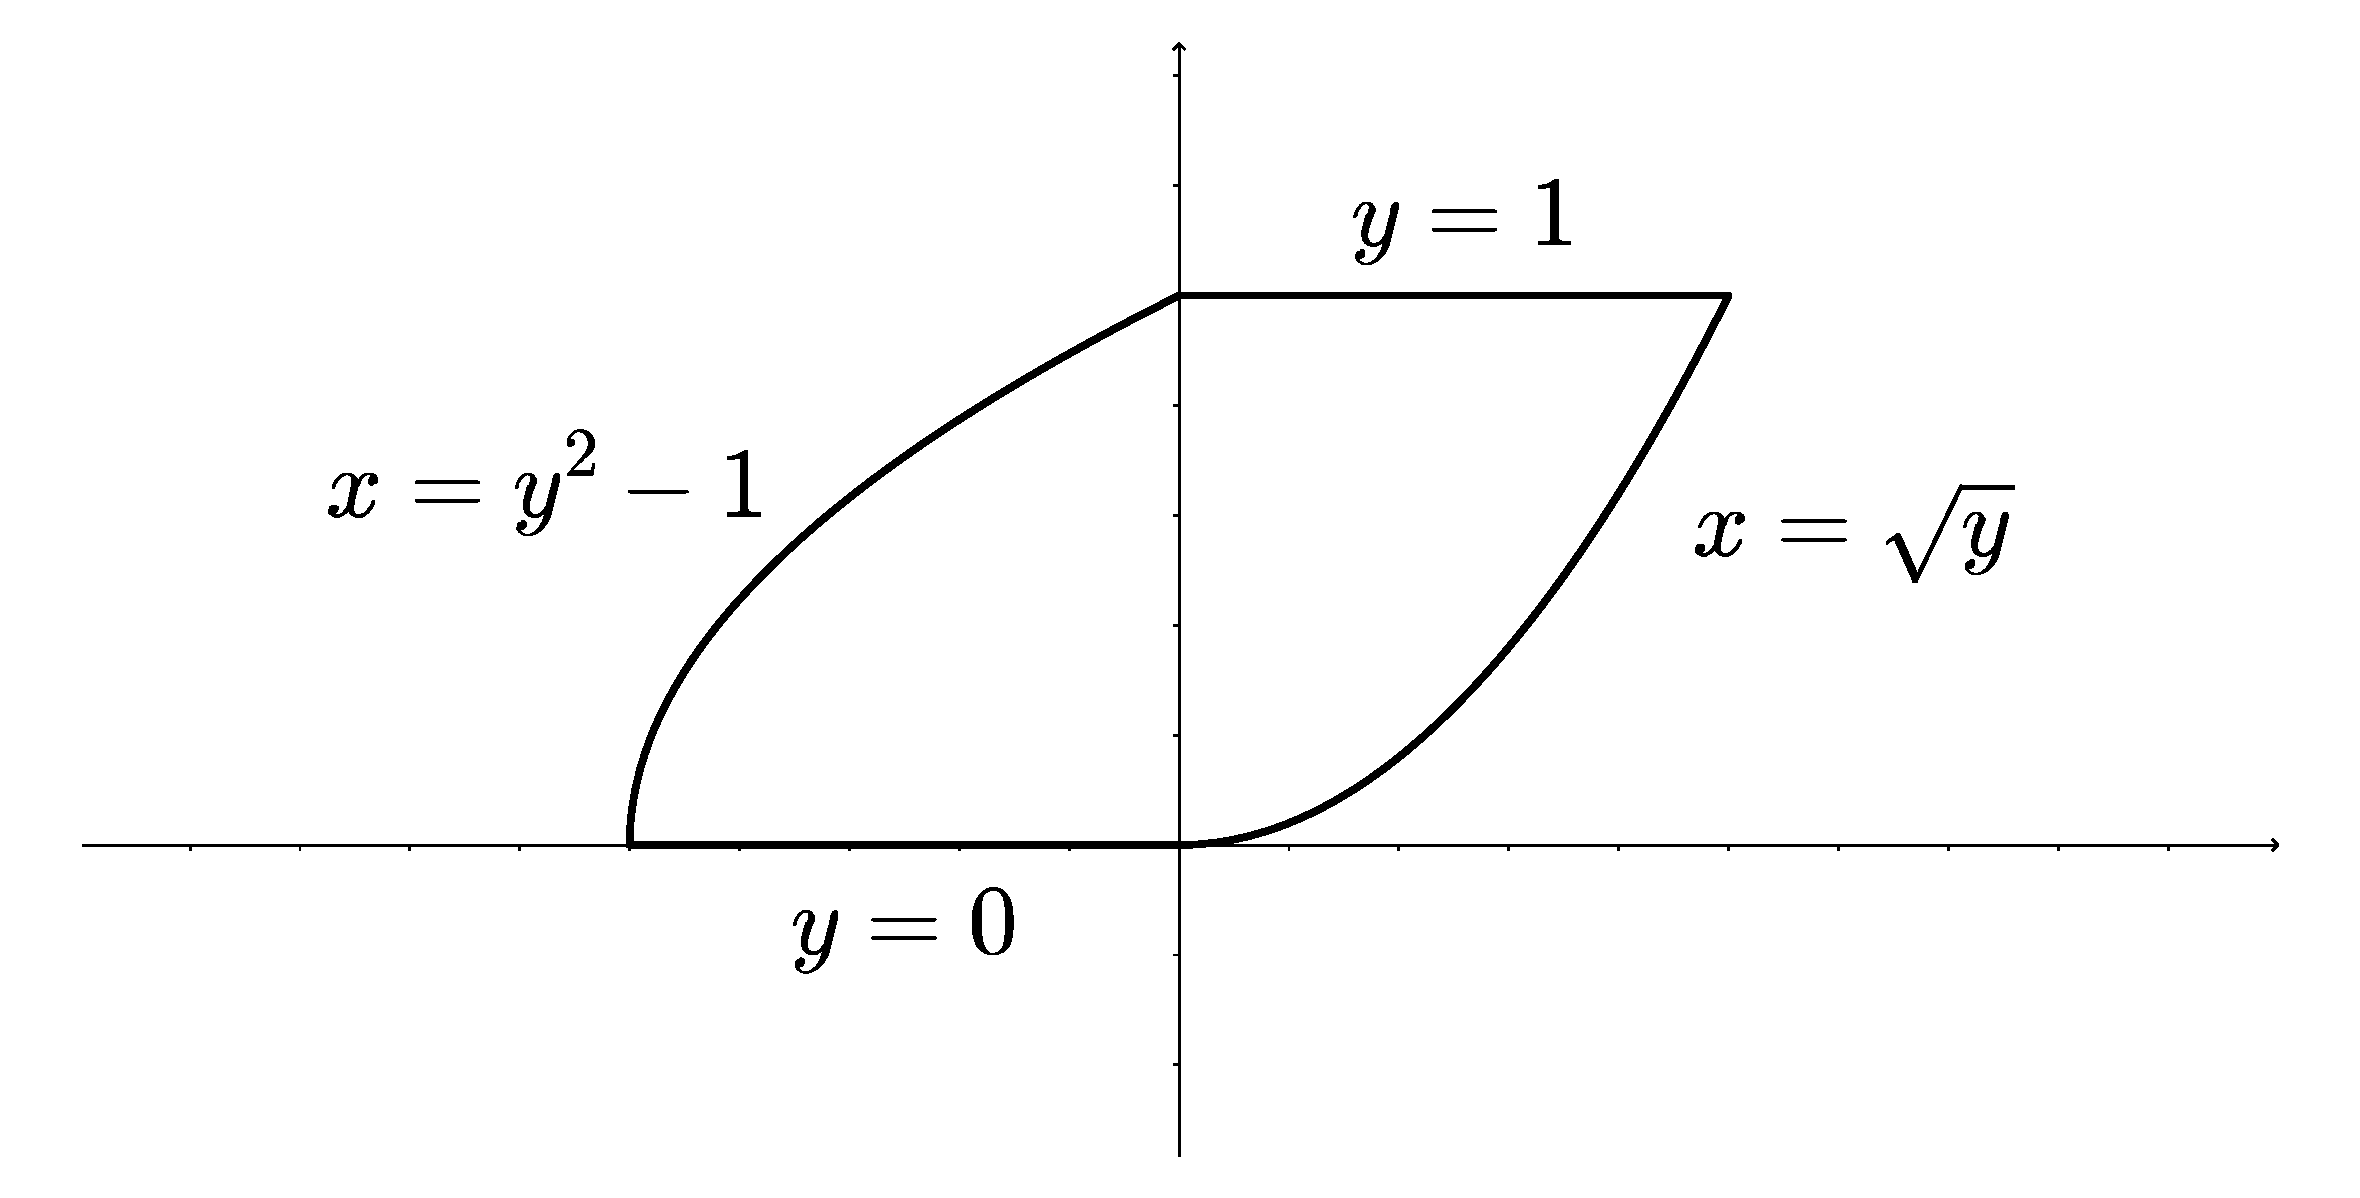
\includegraphics[width=0.4\textwidth]{q3.pdf}
		\end{figure}

	\vspace{0.5cm}
	\item Calcule o volume do s\'olido obtido pela rota\c{c}\~ao da regi\~ao delimitada
		por $y=x^3$, $y=8$ e $x=0$ em torno do eixo $y$.
\end{enumerate}

\vfill{}
F\'ormulas \'uteis:

\[\begin{array}{llll}
	\vspace{0.3cm}
	\cosec(x) = \displaystyle\frac{1}{\sen(x)}, & \sec(x) = \displaystyle\frac{1}{\cos(x)}, & \cotg(x) = \displaystyle\frac{\cos(x)}{\sen(x)}, & \ds\tg(x) = \frac{\sen(x)}{\cos(x)}\\
	\vspace{0.3cm}
	\sen^2(x) + \cos^2(x) = 1, & \tg^2(x) + 1 = \sec^2(x), & 1 + \cotg^2(x) = \cosec^2(x) & \\
	\vspace{0.3cm}
	\sen^2(x) = \displaystyle\frac{1 - \cos(2x)}{2}, & \cos^2(x) = \displaystyle\frac{1 + \cos(2x)}{2} & & \\
	\multicolumn{2}{l}{\sen(x+y) = \displaystyle\sen(x)\cos(y) + \sen(y)\cos(x),} & \multicolumn{2}{l}{\cos(x+y) = \displaystyle\cos(x)\cos(y) - \sen(x)\sen(y)} \\
	& & & \\
	\multicolumn{2}{l}{\sen(x-y) = \displaystyle\sen(x)\cos(y) - \sen(y)\cos(x),} & \multicolumn{2}{l}{\cos(x-y) = \displaystyle\cos(x)\cos(y) + \sen(x)\sen(y)}
\end{array}\]

\begin{flushright}
	\vspace{1cm}
	\textit{Boa Prova!}
\end{flushright}

\end{document}
